\documentclass[../main.tex]{subfiles}
\begin{document}
\label{chap:3}
%cosa significa che la cultura influenza le negoziazioni? --> negoziatori sono persone -> la cultura influenza le persone -> cultura influenza le negoziazioni

%che tipo di cultura? cultura nazionale perché si presume che i negoziatori abbiano circa la stessa cultura lavorativa

%come si studia l'influenza della cultura? -> cerca casi simili ma con risultati diversi
%facciamo una cernita delle fonti? tipo considerare solo bibliografia inglese per esempio?
%\textbf{Culture.}\\
%Culture is a deeply varied, multifaceted concept that embraces many fields. Culture is defined, by the Merriam-Webster dictionary, as "the customary beliefs, social forms, and material traits of a racial, religious, or social group" and also "the set of shared attitudes, values, goals, and practices that characterizes an institution or organization"\cite{definitionculture}. Culture is indeed a broad concept, but, most importantly, culture is not static: it changes and fluctuates over time and space. However, for the purpose of this thesis, the concept of culture will be analyzed under the topic related point of view (??). \\
%da finire!!

Culture is arguably one of the most difficult concepts to delineate. What is culture? How can it be determined? What are its borders? These questions are very complicated to answer. But, for the purpose of this thesis' topic, I will try to define and mark the borders of the concept. But before doing so, some clarifications are in order. For these clarification, I will follow the path of Helen Spencer-Oatey in her article "What is Culture? A compilation of Quotations"(2012), in which she orderly makes some considerations about culture and collects quotations from the most famous scholars; first of them all being Hofstede.

\subparagraph{Even intellectuals are divided on what culture really is.} Therefore, I do not have the presumption to solve this issue: my goal is to have some of the definitions clear and to make a little room for some reasoning on my own. Avruch, in his work, tries to order the definitions of culture in three broad categories. The first one, pioneered by Matthew Arnolds' \textit{Culture and Anarchy} (1867)\footnote{See: Arnold, Matthew. Culture and anarchy. OUP Oxford, 2006.} sees culture as a special intellectual or artistic attempt or product: in this definition, only a small group of people has culture, as it might be referred as "high culture" as opposed to popular culture. In this context, culture refers more to the appearances (that is the looks, the image) of a social group rather than to social sciences itself. Almost as a response to this stream of thought, the second one considers culture as a trait that everybody has which enables people to go from "savagery" to "civilization". The major exponent is Edward Tylor: his definition of culture includes a complexity of elements, such as knowledge, art, law, and capabilities \mancite\autocite[1]{tylor}. The main difference is that all these elements are endowed by every men belonging to a society. Finally, the third way culture has been analysed underlines the uniqueness of cultures across different societies: the main difference with the previous usage is that this approach sees the unique character of culture as opposed to a universal single nature (contained in Tylor's use).

\subparagraph*{Culture is made of layers.} Schein %controlla e cita ammodino la fonte
suggests that it is necessary to make a distinction between the different layers through which culture manifests itself. Those layers are: observable facts, values, and basic underlying assumption (Figure \ref{fig:schein}).
\begin{figure}[h]
    %\centering\includegraphics[width=0.8\textwidth]{images/cafoscari.png}
    \centering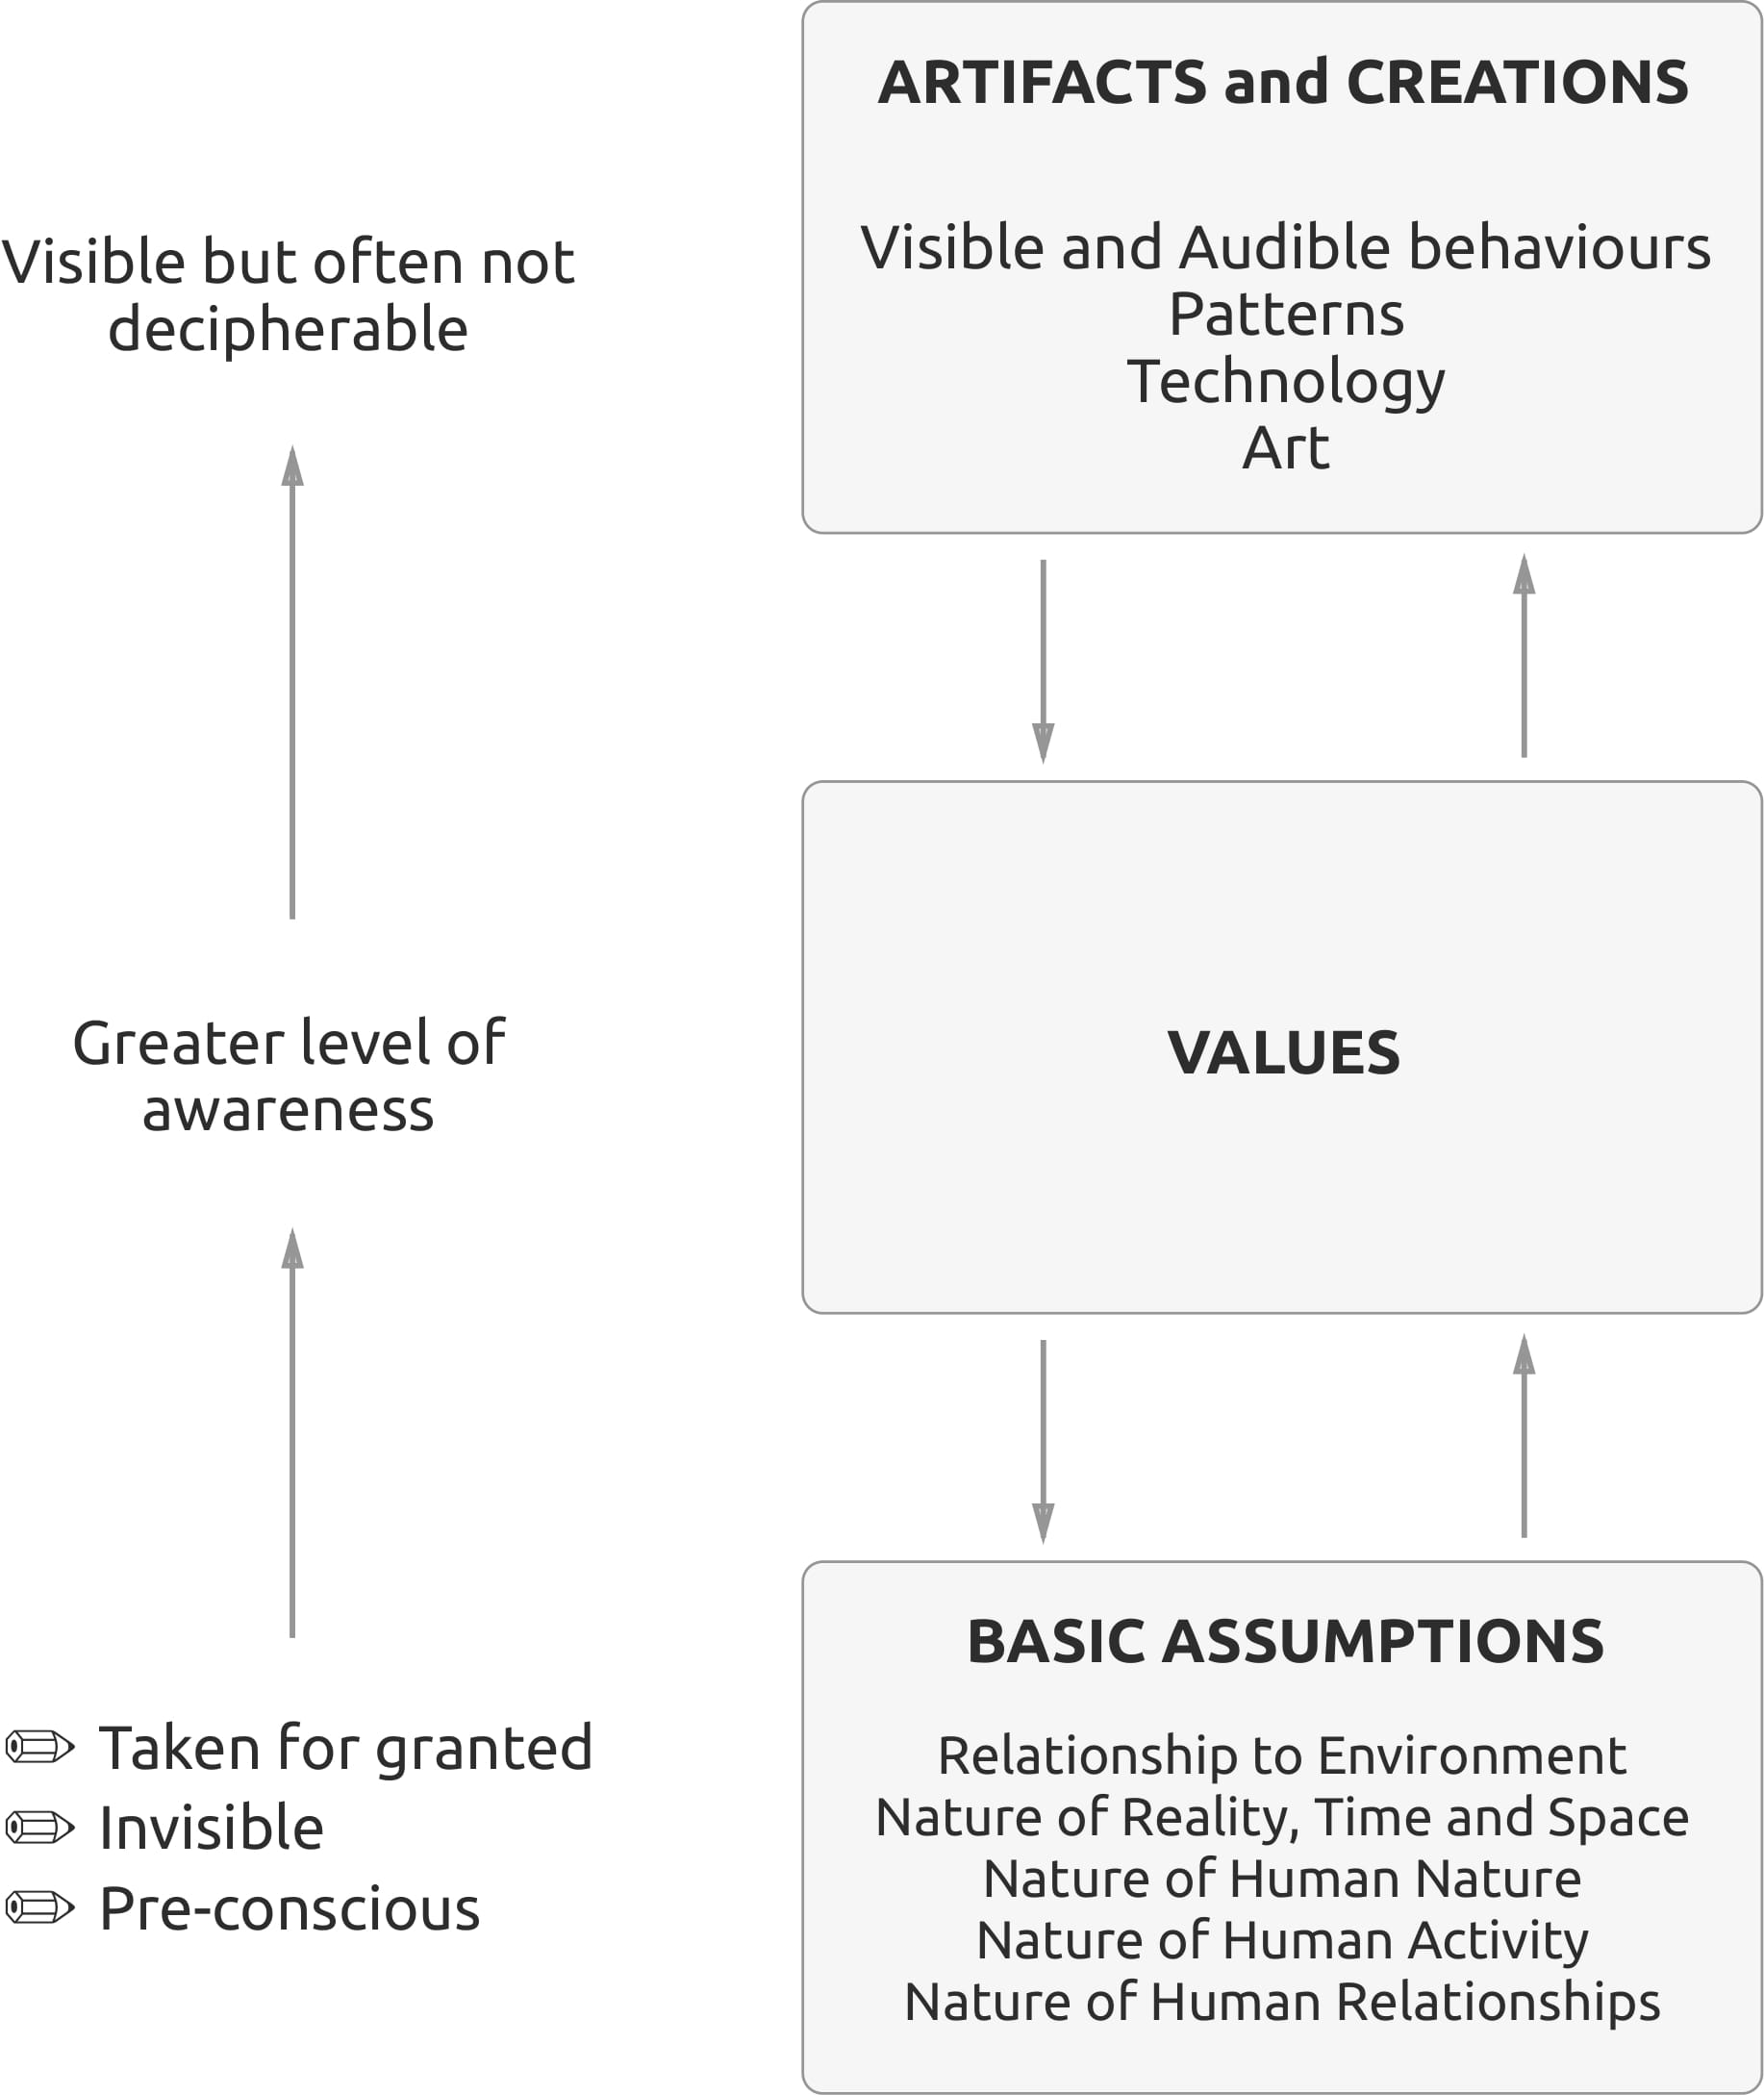
\includegraphics[width=0.7\textwidth]{images/values}
    \caption{Schein's model: levels of culture \autocite[4]{schein}.} %scrivi ammodino la didascalia poi eh
    \label{fig:schein}
\end{figure}

The first one relates to the surface, to what is visible: here data is very easy to acquire but difficult to interpret. To put it in other words, by looking at the observable facts, we can understand "what" are the behavioural norms followed and "how" the group builds the surroundings, but we cannot understand "why" a group adopts a specific behaviour. To answer the question of "why" a group of people adopts certain behaviours, we need to take into consideration the values, that compose the aforementioned second layer. However, values represent only the espoused values of a culture: this means that they unveil only what people \textit{say} it is the reason for their actions. Therefore, the real motivations remain obscure or unconscious. To solve this issue, it is necessary to appeal to the basic underlying assumptions. Those assumptions are themselves a sort of learned responses that were originally espoused values \autocite[3]{schein}. However, as values lead to a certain behaviour and behaviours are a manifestation of a culture, values turns into an underlying assumption about how things really are. Once the assumption is established and, therefore, taken for granted, it abandons consciousness. Assumptions that are taken for granted are powerful because are less keen to be a subject of debate than espoused values. When dealing with an underlying assumption, it will be hard to find someone willing to discuss the reason behind it. For example, the belief that a business should be profitable is something that we assume is the right way of doing business but actually we cannot explain exactly when we learned that notion, we just know it. The result of Schein suggestion is that, in order to visualise the effects of culture on international negotiations, it is necessary to search for the behaviours, then the values, and, eventually, those will lead to the underlying assumptions \mancite\autocite[4]{schein}.%qui metti citazione schein

\subparagraph*{Culture can even influence biological processes.} Ferraro theorises that culture influences biological processes. Indeed, the vast majority of conscious behaviours are learned through interaction with other members of our culture. Culture does not influence our biological needs because everyone needs to eat, drink, sleep regardless of their culture. But it does influence how we eat, how often, with whom, how much, and according to which rules. The effects of culture on the natural processes of the body varies across cultures and forms. For example, in certain cultures, the internalised idea is that through a series of specific respiration techniques it is possible to later the experience of pain \footnote{For example, the Fiji firewalkers, or the Cheyenne men actively involved in the Sun Dance ceremony where men fast for days and get their chests pierced.}.

\subparagraph*{Culture can be discerned between universal human nature and unique individual personality.} As Hofstede points out, culture is learned not inherited. This is a very important remark because it implies that culture does derive from the social environment and it is not something that comes from the genes. Moreover, culture should be differentiated in human nature, on one side, and in an individual's personality, on the other. Nonetheless, the border between those two concepts is very blurry and it is still object of discussion. Hofstede identifies three levels of uniqueness in the human mental programming (Figure \ref{hofstede}):
\begin{figure}[h]
    %\centering\includegraphics[width=0.8\textwidth]{images/cafoscari.png}
    \centering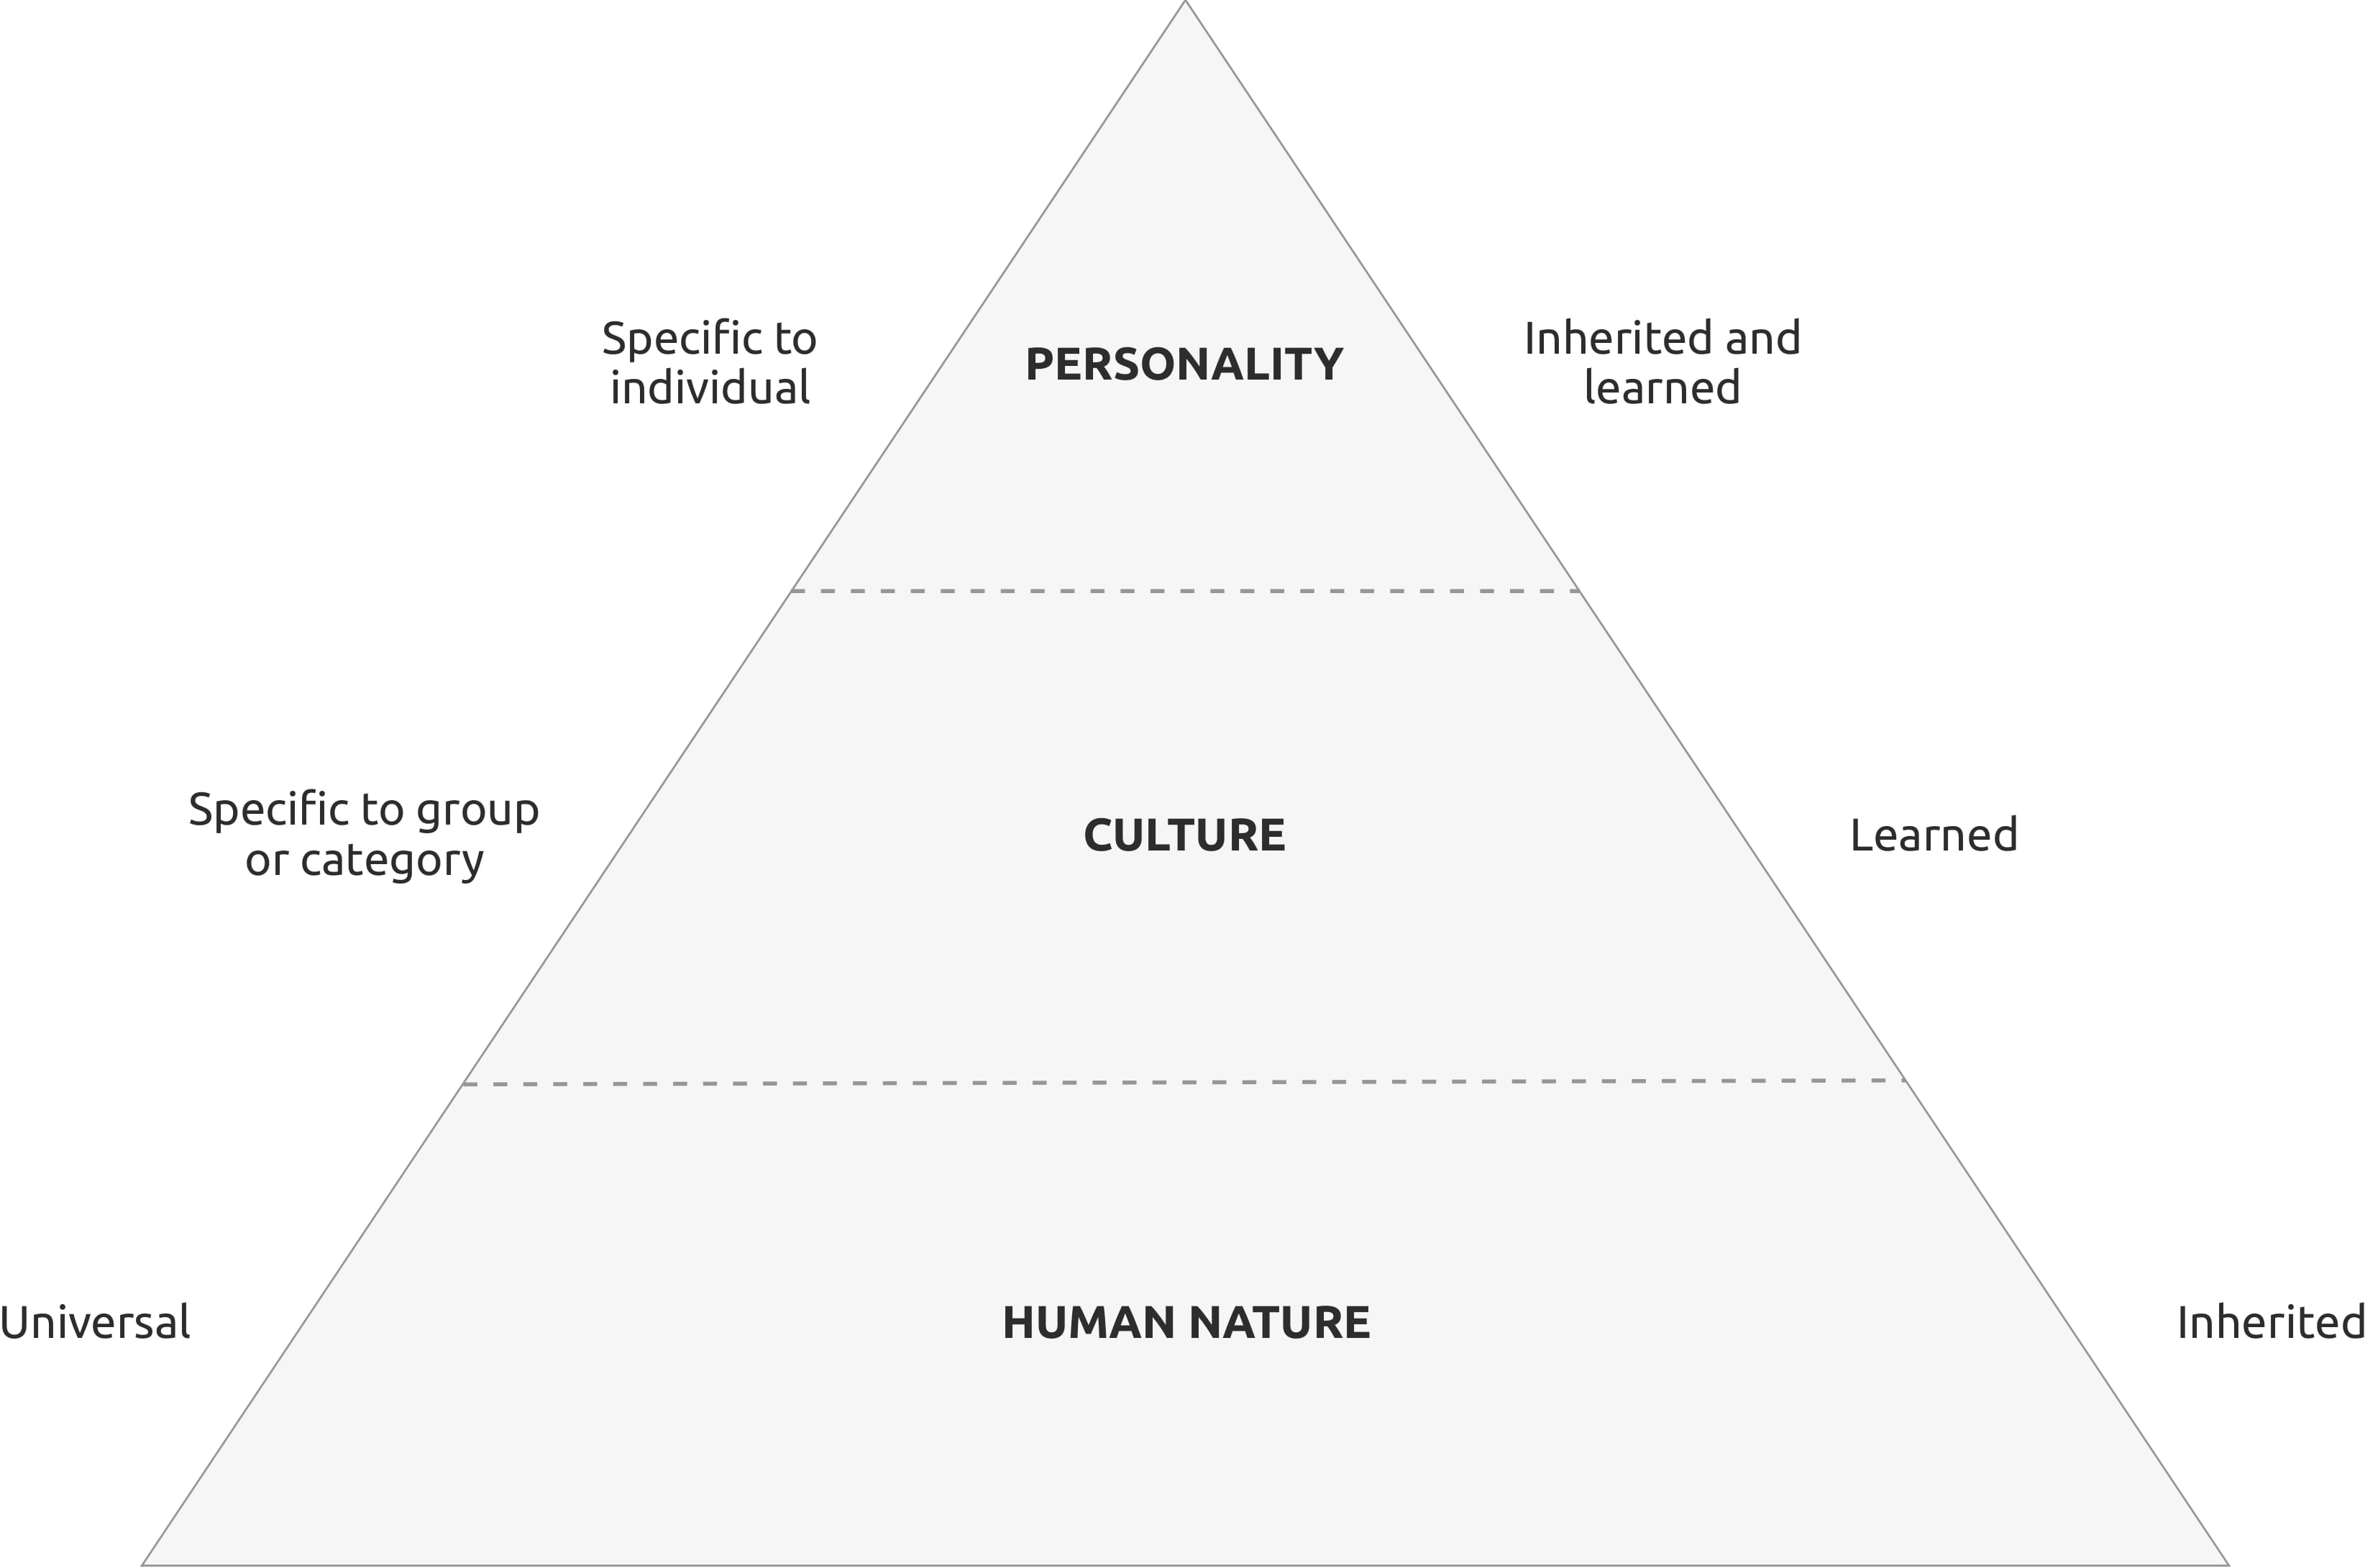
\includegraphics[width=0.85\textwidth]{images/levels-1}
    \caption{Hofstede's model: levels of mental programming \autocite[6]{hofstede}.}
    \label{hofstede}
\end{figure}

\textit{Human nature} is maybe the only thing that all human beings have in common: this level is inherited from one's genes and it relates to one's physical and basic psychological functioning. For example, the human ability to perceive feelings or the basic needs, such as the need to associate with others. However, the way in which the feelings are expressed and how an individual associates with others is affected by culture. Most of the aspects related to this level concern also the animal kingdom when there is a reference to primal instincts. On the other hand, the \textit{personality} of an individual is their personal set of mental programming that do not share with anyone else. It is a combination of human nature deriving from one's genes and of something learned through both culture and personal experiences. Historically, cultural assets have been linked with heredity because scholars could not find a better explanation for the outstanding differences in cultural patterns among different civilisations. But, the role of hereditary has been amplified in the "theories" about race which somehow have been used to justify, over the course of history, cultural superiority and inferiority\footnote{It is sufficient to think about how the feeling of being a "superior" race led to despicable events, such as the Holocaust, the Apartheid, the racial laws that existed in the US against African-American people.}.
%qui metti citazione hofstede ammodino!!

\subparagraph*{Culture is associated with social groups.} Both Ferraro and Hofstede sustain this statement. Indeed, culture is \textit{shared} between two or more people. In other words, there cannot be a culture of an eremite. Returning to the aforementioned Hofstede's scheme of mental programming (Figure \ref{hofstede}), he suggests that each individual belongs to different groups and categories at the same time. Therefore, as a consequence, each person bears different layers of mental programming corresponding to different levels of culture. Those levels are:
\begin{itemize}
\item National level according to one's country (or \textit{countries} for people who migrated);
\item Regional/ ethnic/ religious/ linguistic affiliation (as most nation are composed of culturally different groups);
\item Gender level;
\item Generation level, which separates different kin generations;
\item Role category (e.g. parent, son/daughter, teacher, student);
\item Social class level, associated with educational opportunities and with a person's occupational profession;
\item Organisational or corporate level, according to the way employees have been socialised within their working environment. \autocite[18]{hofstede}
\end{itemize}
Hofstede also notes that, especially in modern society, many layers are in conflict with each other. For example, religious values may conflict with generation values. As a result of these conflicts in mental programming, anticipating the behaviour of people in a new situation gets challenging.

This last distinction was also made by Salacuse %e qui citi ammodino
when distinguishing between national and professional culture in his article "Ten ways that Culture Affects Negotiating Style: Some Survey Results" (1998). In his article, he defines culture as "the socially transmitted behaviour patterns, norms, beliefs and values of a given community." \autocite[222]{salacuse}. Indeed, for the purpose of his article, he makes a distinction between national culture and professional or occupational culture. The professional %magari cerca un sinonimo
background forms a subculture of some sort, therefore it is necessary to take it into consideration.

In his article, he takes on a survey and analyses both national and professional culture of the participants (the nature of the article will be discussed in details in the next chapter).

Professional culture, or organisational culture, is the mental programming layer most discussed among the different layers of culture embedded in one's mind. Rohit Deshpande and Frederick E. Webster, in their article "Organizational Culture and Marketing: Defining the Research Agenda" (1989), give a clear yet simple and understandable definition of what organisational culture is. They define it as "the pattern of shared values and beliefs that help individuals understand organisational functioning and thus provide them norms for behavior in the organization" \autocite[4]{rohit}.

Avruch intervenes in this context because he provides us with an explanation of the reason why it is necessary to have the notion of "subculture". In his book "Culture and Conflict Resolution"(1998), he sustains that since individuals are organised in many potential different ways within a population, by many different criteria, the more complex and differentiated the social system is, the more potential groups and institutions there are. As a consequence, each of these groups and institutions can be potential containers for culture. Hence, no population can be characterized as a single culture, but it will be a complex of \textit{subcultures} \autocite[18]{avruch}. %controlla citaz

For the purpose of this thesis, however, these distinctions concerning the different layers of mental programming (in Hofstede's words), or concerning the concept of subculture (in Avruch's words) will not be contemplated as, in an international diplomatic negotiation, the negotiators are thought to belong (more or less) to the same professional, generational, social class background. Therefore, the cultures that are taken into consideration in this work are the one belonging to a country\footnote{For the scope of this work, a country is considered an homogeneous entity enclosed within its current political border.}. From now on, the focus will be on national culture (mentioned as just culture).

\subparagraph*{Culture is both an individual construct and a social one.} In this context, Matsumoto provides us with his contribution: according to him, "culture is as much an individual, psychological construct as it is a social construct"\autocite[18]{matsumoto}. The degree with which an individual absorbs the norms and values of the culture they belong produces a unique individual culture. Historically, this distinction, this nuanced way an individual could absorb a culture was not taken into consideration and often led to the creation of stereotypes.

\subparagraph*{The delineation of a culture's features will always be fuzzy as they are both socially and psychologically distributed in a group.} Here Avruch helps us with his reasoning. Indeed, almost as a consequence of the previous point, since each individual will absorb cultural norms with a different degree, two individuals cannot share perfectly the same cultural contents. As a result, culture is socially distributed within a population \autocite[18]{avruch}. Furthermore, also cultural representations are internalised by individuals. Also in this case, they do not internalise representation in the same way. Some individuals will embrace representation in a superficial way, some others will embrace them more deeply. It goes without saying that the deeper is the internalisation, the more individuals will be motivated to actions. Therefore, the same cultural representation might be internalised differently by two individuals. This results in a non uniform distribution of culture: hence, culture is psychologically distributed within a population \mancite\autocite[20]{avruch}.

\subparagraph*{Culture has both unique and universal characteristics.} A universal characteristic might be the concept of social distance\footnote{The concept of \textit{social distance} was introduced by anthropologist Edward T. Hall: he was the pioneer of \textit{proxemics}, that is the study of space. His work will be analyzed in the next chapter.} for example, but how it is treated and how it is expressed depends uniquely on the culture: some cultures base social distance on race, some others on social classes, etc. Matsumoto brings the example of eye gazing in social situations. Gaze behaviour differs across cultures: indeed, cultures have different rules regarding the appropriateness of gazing at others when interacting with them. What is the universality here? In social situations, the most common reason is to show politeness. However, cultural rules will lead to different behavioural expression to deliver politeness. For example, in Western cultures it is considered polite to look directly in the eyes of whom you are talking to. On the other hand, in Eastern cultures, it is required \textit{not} to look directly in the eyes of your interlocutor in order to show politeness and respect \autocite[21-22]{matsumoto}. In other words, the observable behaviours indicate the unique traits of a culture, meanwhile in the reasons for those behaviours lies the universality of cultures. And this is how the uniqueness and the universality of culture can coexist in relation to our behaviours.

\subparagraph*{Culture is learned.} As we mentioned before, culture is learned through the people you interact with. Ferraro informs us that this concept causes many implications. First, saying that culture is learned implies that an individual can also learn about other cultures: this will lead to a greater tolerance and understanding, therefore leading to a better communication with others. Second, since we learn culture, it is possible for an individual not only to function in their own culture, but also in other cultures. Third, foreign work forces lacking certain job related skills are capable to learn those skills in the future \autocite[19]{ferraro}.

\subparagraph*{Culture is a descriptive concept.} Culture describes the ideas and norms shared by a group of people: hence, the concept of culture does not have an evaluative nature. Historically, some scholars have been linking the concept of culture with "well educated", "refined", "cultured". But this definition might provoke the feeling that there are "high cultures" and "low cultures", or that there are some advanced cultures and some backwards cultures. The concept of culture is not judgemental. It just tells us that there are cultures similar or different from each other.

\subparagraph*{Culture is subject to gradual change.} The one thing that we can all agree on is that culture changes. We cannot think that culture is a static concept.
It is essentially fluid and constantly in motion. This makes it so that it is difficult to define any culture in only one way in the first place. Ferraro \autocite*[25-29]{ferraro} helps us once again to understand better this concept. First of all, mechanisms of change within a culture are called \textit{discovery} and \textit{invention}. Nonetheless, most innovations introduced into a culture are the result of borrowing from other cultures. This process is called cultural \textit{diffusion}, meaning the permeating of cultural elements from one culture to another.

Why this happens? It is merely an explanation in term of economy of effort: indeed, it takes less effort to borrow someone else's invention rather than making it from scratch. Cultural diffusion varies from situation to situation but there are some stable elements worth mentioning.

First, cultural diffusion is a selective process. This means that cultures do not borrow every item from other cultures indistinctly. If so, the difference among cultures would have eventually disappeared. Rather, cultures borrow from other cultures the items useful for them and that result compatible with their own characteristics. Therefore, an item will be taken into consideration if it is seen superior to the existing one, it is consistent with the cultural pattern, it is easily understandable, it can be tested on an experimental basis, and it provides clear benefit that can be seen from a large group of persons.

Second, culture diffusion is a reciprocal process. It means that when two cultures get in touch with each other, \textit{both} cultures will borrow something from the other.

Third, it is very rare that the items cultures borrow from other cultures are embedded within the culture in the original form. Every item goes through a process of reinterpretation in order for it to be more effectively and more efficiently integrated into the total configuration of the borrowing culture. As an example, let us take into consideration the food par excellence: pizza. Pizza is notoriously a wide-world recognized Italian dish, however it has been adopted by cultures all over the world. Originally, pizza is made with mozzarella, tomato sauce, oregano, on a crust made of water, flour, oil, and yeast. However, in some cultures, oregano is considered too spicy, therefore the dish has been reinvented to meet the taste of other cultures. In some countries it is topped with processed cheese instead of mozzarella and the oregano has been left out. Or in some other occasions, the toppings chosen are very far from the original ones. Such as the choice of putting pineapple on pizza. Even if an Italian person would not recognize as legitimate a pizza with pineapple on it, they would still call it pizza.

\begin{figure}[h]
\centering
\begin{subfigure}{.5\textwidth}
  \centering
  
\includegraphics[width=.53\linewidth]{images/margherita.png}
  \caption{Pizza.}
  \label{fig:sub1}
\end{subfigure}%
\begin{subfigure}{.5\textwidth}
  \centering
  
\includegraphics[width=.5\linewidth]{images/hawaii.png}
  \caption{"Pizza".}
  \label{fig:sub2}
\end{subfigure}
\end{figure}

Fourth, some cultural traits are more easily diffused than others. Logically, technological innovations are more likely to be borrowed than social patterns. For instance, it is easier to convince a man that a car will carry you faster than by walking on foot; however, it will be more difficult to convince a Hindu person to switch to socialism.\\

\textbf{Misconceptions about culture.}

Now that the key characteristic of culture have been presented and analysed, Avruch and Hofstede's reasonings suggest that it is necessary to mention some misconceptions related to the notion of culture. More than misconception, the following list relates to ideas about culture we could define inadequate.

\textit{Culture is homogeneous}. This statement presupposes that a culture is free from internal paradoxes. In particular, it implies that a culture provides clear and unambiguous "instructions" on how to act; moreover, it implies that once that culture is learned by an outsider, it can be characterised in a "straightforward" way.

\textit{Culture is a thing.} Conceptualising culture as a thing may lead to think about culture as something that can act on its own, independently from human actors. But by making it a thing, it is possible to forget about intracultural diversity.

\textit{Culture is uniformly distributed among members of a group.} If this was true, every member of the group would be uniform under cognitive, affective, and behavioural aspect. Intracultural differences are once again ignored.

\textit{An individual possesses but a single culture.} In this case, culture coincide with group identity. This misconception comes from the fact that in the first studies about the subject, anthropologists would select small ethnic group which seemingly had one common culture. Then, political scientists expanded the unit of analysis from a small ethnic group to a nation-state, hence the national characterisation. As Hofstede and others told us, an individual carries multiple cultures.

\textit{Culture is custom.} By simplifying culture as mere customary behaviours, we reduce culture as a surface-level etiquette. Therefore, in this sense, culture is structurally undifferentiated and individual agency is devalued.

\textit{Culture is timeless.} This misconception asserts culture as unable to change in quality over time. Culture is something that is at the same time above time and under the influence of time. It is something that was there before our time and, at the same time, it is influenced by current times and it constantly changes. Culture is indeed shaped by what is in the present but also carries what it took from the past \autocite[14-16]{avruch}.

\textit{Culture and identity are the same thing.} Identity answer the question: Where do I belong? Identity is based on the images and stereotypes we have of other culture, but for this reason it only scrapes the surface. Two populations might fight each other on the basis of different identities and yet share the same values. Identity also differs in relation to the context: indeed, a shared identity needs a shared other. In my home country, I feel Italian and I can tell the difference with other European countries, but when in the US or in Asia, we all feel Europeans \autocite[10]{hofstede2001}.\\

In other words, culture is intricate, yet intuitive. It has many aspects to be acknowledged in order to have a at least a partial conception of it. However, some remarks are important to make, in order to keep going with this work. Culture has many layers, as it can relate to gender, age, professional environment, social class. But, as stated before in this chapter, as the focus in on negotiations, negotiators are thought to belong to the same (or almost the same) group concerning age, social class, professional environment. Therefore, what matters, what stands out is the difference in national cultures. In recent times, though, with globalisation, it is easier to see that cultures are diffusing among them, meaning that they borrow traits and inventions from one another and this leads to some sort of homogenisation concerning some aspects.
The most important thing for the purpose of this thesis is to realise that culture can be learned. Indeed, when confronting a party from another culture, a negotiator can learn about the other party's culture and be prepared for differences and divergences. Hence, it is possible to restrain potential disagreements. What is important to remember is that the intentions of the negotiators are all the same: to reach an agreement in the smoothest way. The issue come when it is time to manifest the actions in order to reach the desired effect. That is when culture does its part and leads to different approaches and behaviours.

For the purpose of this thesis, this analysis of culture is sufficient to understand what relies under this notion. It is, indeed, a very broad, rich, varied conception which still today causes debates over its nature, its definition, its characteristics. But, as much as it is an interesting and fascinating debate, the clarifications made in this chapter are enough for the usefulness of this thesis.

\end{document}